\section{Application 1: Whitening Variational Gaussian Processes}
\label{sec:variational_results}

Assume we have $M$ inducing points $\bZ = [\bz_1, \ldots, \bz_m]$.
Let $q(\bu) = \normaldist{\bu; \bm}{\bS}$ be the approximate function distribution at the inducing points $\bZ$.

For an arbitrary point $\bxtest$, the predictive distribution for the approximate Gaussian process is given by
%
\begin{equation}
  q \left( f(\bxtest) \right) = \Evover{q(\bu)}{ \: p\left( f(\bxtest) \mid \bu \right) \: }
  = \normaldist{ \bxtest; \ameantest{ \bxtest }} { \avartest{ \bxtest }}
  \label{eqn:approx_pred}
\end{equation}
%
where $\ameantest{\cdot}$ and $\avartest{\cdot}$ are the (approximate) predictive mean and covariance functions, given by:
%
\begin{align}
  \ameantest{\bxtest} &= \bk_{\bZ\bxtest}^\top \bK_{\bZ\bZ}^{-1} \bm
  \label{eqn:approx_pred_mean} \\
  \avartest{\bxtest} &= k(\bxtest, \bxtest) -
    \bk_{\bZ\bxtest}^\top \bK_{\bZ\bZ}^{-1} \left( \bK_{\bZ\bZ} - \bS \right) \bK_{\bZ\bZ}^{-1} \bk_{\bZ\bxtest}
  \label{eqn:approx_pred_covar}
\end{align}
%
We learn the parameters $\bm$ and $\bS$ (as well as the inducing locations $\bZ$ and associated kernel/likelihood hyperparameters) through gradient-based optimization.
We can either optimize the evidence lower bound \cite{hensman2015scalable} for variational inference or the predictive log likelihood \cite{jankowiak2020parametric} for regularized maximum likelihood estimation:
%
\begin{align}
	-\loglik_\text{ELBO} &= -\sum_{i=1}^N \Evover{q(f(\bx^{(i)}))}{  \: \log p( y^{(i)} \mid f(\bx^{(i)}) ) \: } + \kl{ q(\bu) }{ p(\bu) },
	\label{eqn:elbo}
	\\
	-\loglik_\text{Pred.} &= -\sum_{i=1}^N \: \log \Evover{q(f(\bx^{(i)}))}{  \: p( y \mid f(\bx) ) \: } + \beta_\text{reg} \kl{ q(\bu) }{ p(\bu) }.
	\label{eqn:predll}
\end{align}
%
For the predictive log likelihood $\loglik_\text{Pred.}$ the $\beta_\text{reg}$ term is a tunable hyperparameter which controls the amount of regularization.



\subsection{The Whitened Parameterization}

Expanding the KL divergence term in \cref{eqn:elbo,eqn:predll} gives us
%
\begin{equation}
	\kl{ q(\bu) }{ p(\bu) } = \frac{1}{2} \Bigl( \bm^\top \bK_{\bZ\bZ}^{-1} \bm + \tr{ \bK_{\bZ\bZ}^{-1} \bS } - \log \vert \bK_{\bZ\bZ}^{-1} \bS \vert - M \Bigr).
	\label{eqn:kldiv}
\end{equation}
%
%The KL divergence is minimized when $\bm = \bzero$ and $\bS = \bK_{\bZ\bZ}$.
This term can cause optimization challenges because the $\bm$ and $\bS$ parameters will need to adapt to changes in $\bK_{\bZ\bZ}$ as the kernel hyperparameters and inducing point locations are optimized.
A solution to this challenge is to perform optimization in the \emph{whitened coordinate space} \cite{matthews2017scalable}.
\[ \bu' = \bR^{-1} \bu, \]
where $\bR$ is a matrix such that $\bR \bR^\top = \bK_{\bZ\bZ}$.
In this coordinate system, note that $p(\bu') = \normaldist{ \bu'; \bzero}{\bI}$.
If we directly optimize the \emph{whitened parameters} $\bm' = \bR^{-1} \bm,$ $\bS' = \bR^{-1} \bS \bR^{-\top},$
the resulting KL divergence becomes
%
\begin{equation}
	\kl{ q(\bu') }{ p(\bu') } = \frac{1}{2} \Bigl( \bm^{\prime \top} \bm' + \tr{ \bS' } - \log \vert \bS' \vert - M \Bigr).
	\label{eqn:kldiv_whitened}
\end{equation}
%
This term does not depend on $k(\cdot,\cdot)$ or $\bZ$, which makes optimization much more stable.
Under the whitened coordinate system, the predictive mean and variance of \cref{eqn:approx_pred_mean,eqn:approx_pred_covar} become
%
\begin{align}
  \ameantest{\bxtest} &= \bk_{\bZ\bxtest}^\top \bR^{-\top} \bm'
  \label{eqn:approx_pred_mean} \\
  \avartest{\bxtest} &= k(\bxtest, \bxtest) -
    \bk_{\bZ\bxtest}^\top \bR^{-\top} \left( \bI - \bS' \right) \bR^{-1} \bk_{\bZ\bxtest}
  \label{eqn:approx_pred_covar}
\end{align}
%
In practice, it is common to set $\bR$ to the Cholesky factor of $\bK_{\bZ\bZ}$.
It is worth noting that all possible choices of $\bR$ are equivalent up to an orthonormal rotation.
\gp{Jake/David: pretty sure I convinced myself this is true, but confirm plz.}

\begin{figure}[t!]
  \centering
  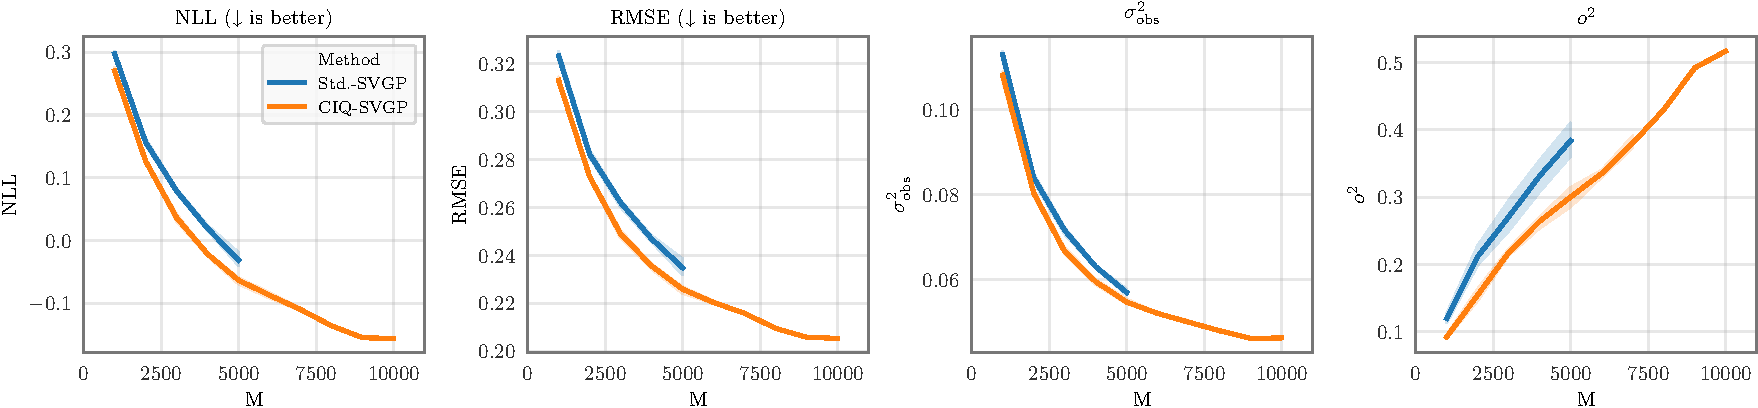
\includegraphics[width=\linewidth]{figures/3droad.pdf}
  \caption{
    SVGP models trained on the 3D-Road dataset ($D=2$, $N\geq300,\!000$), varying $M$ (the number of inducing points).
    \gp{FINISH}
  }
  \label{fig:3droad}
\end{figure}

\begin{figure}[t!]
  \centering
  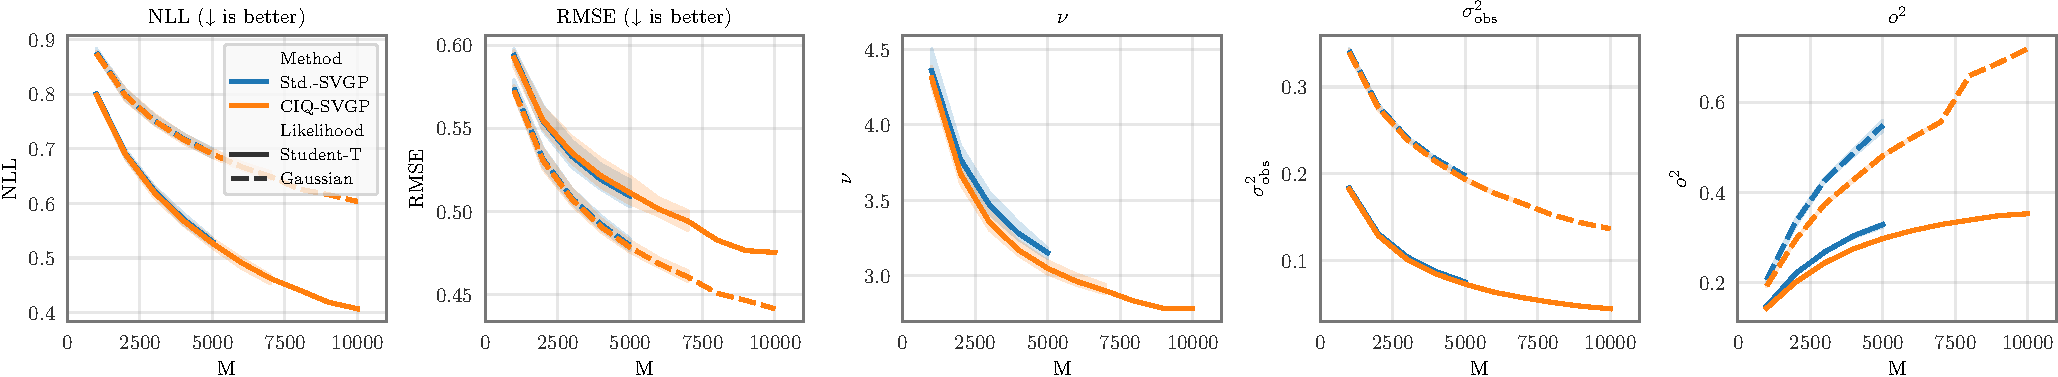
\includegraphics[width=\linewidth]{figures/precip.pdf}
  \caption{
    SVGP models trained on the Precipitation dataset ($D=3$, $N\geq300,\!000$), varying $M$ (the number of inducing points).
    \gp{FINISH}
  }
  \label{fig:precip}
\end{figure}

\begin{figure}[t!]
  \centering
  \caption{
    SVGP models trained on the Robotics dataset ($D=?$, $N\geq?$), varying $M$ (the number of inducing points).
    \gp{FINISH}
  }
  \label{fig:robotics}
\end{figure}
